\documentclass[a4paper,11pt]{kth-mag}
\usepackage[T1]{fontenc}
\usepackage{textcomp}
\usepackage{lmodern}
\usepackage{datetime}
\usepackage[utf8]{inputenc}
\usepackage[swedish,english]{babel}
\usepackage{modifications}
\usepackage{graphicx}
\usepackage{subcaption}
\usepackage{url}
\selectlanguage{swedish}
\title{Benchmarking Human Solving Methods for
           Rubik's cube}

\subtitle{Duis autem vel eum iruire dolor in hendrerit in
          vulputate velit esse molestie consequat, vel illum
          dolore eu feugiat null}

\author{Andreas Nilsson  anil9@kth.se\\Anton Spång  aspang@kth.se}
\date{\today}

\blurb{DD143X - Bachelor Thesis\\Supervisor: Michael Schliephake\\Examiner: Örjan Ekeberg}
\trita{TRITA xxx yyyy-nn}
\begin{document}
\frontmatter
\pagestyle{empty}
\removepagenumbers
\maketitle
\selectlanguage{english}
\begin{abstract}
  This is a skeleton for KTH theses. More documentation
  regarding the KTH thesis class file can be found in
  the package documentation.


\end{abstract}
\clearpage
\begin{foreignabstract}{swedish}
  Denna fil ger ett avhandlingsskelett.
  Mer information om \LaTeX-mallen finns i
  dokumentationen till paketet.
\end{foreignabstract}

\clearpage
\tableofcontents*
\mainmatter
\pagestyle{newchap}
\chapter{Introduction}
\begin{figure}
	\centering
	\begin{subfigure}[b]{0.3\textwidth}
		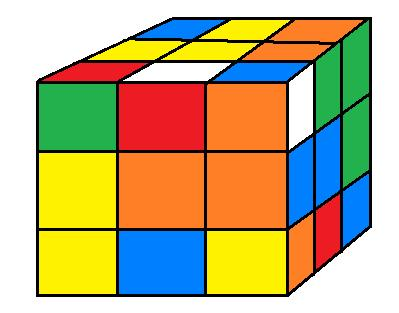
\includegraphics[width=\textwidth]{figs/scramble.jpg}
		\caption{Scrambled cube}
	\end{subfigure}
	\begin{subfigure}[b]{0.3\textwidth}
		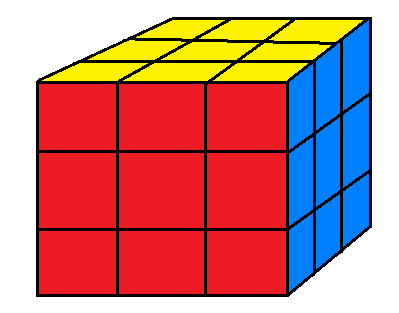
\includegraphics[width=\textwidth]{figs/DONE.png}
		\caption{Solved cube}
	\end{subfigure}
\end{figure}
The Rubik’s cube is an 3-D combination puzzle, where each side of the cube is covered with nine squares in six possible colours: white, red, blue, orange, green and yellow.\\
You start with a scrambled cube, meaning that the colored miniature cubes (also known as cubies) are randomly positioned by using random operations on the cube (fig 1) . \\
The goal is to obtain each side of the cube covered with only one colour per side, which is the unique solution (fig 2). 
Different methods have been developed with series of notation to solve subproblems, one at the time to reach the unique solution. The general idea which many methods are based on is to solve it one layer at the time.\\
If you were to randomly rotate the faces in an attempt to solve the cube, there is almost zero chance of achieving the solved state in your lifetime because of all the possible permutations of the cube. There are $4.3 * 10^(19)$ (or 43 quintillion) [8] different states. Assuming you get to a unique state every second it would take more than 130 billion years to test 10\% of the cubes possible states [appendix A].\\
There are two major ways to compete in solving the Rubik’s cube: the least amount of moves and solving the cube as fast as possible (speedcubing).
The cube was invented by the professor of architecture Ernő Rubik as a teaching tool to help his student understand 3D objects. It was not until he scrambled his new cube and tried to restore it, that he realize that his creation was a puzzle.\\ 
The cube was originally called magic cube and was licensed to be sold by the american toy company Ideal Toy Company in 1980. [13].


\section{Problem Definition}
This thesis will explore two commonly known beginner methods for human solving of rubik’s cubes. Both based on the idea to solve the cube one layer at the time which is the easiest way for the human mind to solve this kind of problem [2]. To find the most effective for speedcubing and least amount of moves we will evaluate both methods operation variance, number of operations and time.\\

During the literature study there was no such comparison of solving-methods for 3x3x3 cube found. The information found about solving-methods for 3x3x3 cubes was tutorials of how to use them.

\section{Problem Statement}
Which of the beginner algorithms would be more effective for speedcubing?\\
Which of the beginner algorithms solves the cube with the least amount of moves?\\
Which beginner algorithm is easiest to learn and execute to someone inexperienced with the cube?\\
\section{Purpose}
\section{Structure}
The second section will introduce the reader to concepts necessary to understand the algorithms implemented and benchmarked. The third section will explain the methods used in this thesis. The fourth sections will explain the implementations made in detail and the difficulties.\\
The fifth section will be for presenting the results and the sixth section for discussion regarding the results. After that will there be a conclusions section that completes the circle of the thesis, answering the problem statements. Lastly the references used to this thesis will be listed followed by appendix containing computations and graphs.   


\chapter{Background}
\section{Competitions}
\subsection{Speedcubing}
\subsection{Fewest moves}
\section{Rubik's Cube}
\subsection{Description}
\subsection{Notation}
\section{Algorithms}
\subsection{Lbl using daisy method}
\subsubsection{White cross}
\subsubsection{White corners}
\subsubsection{Middle layer edges}
\subsubsection{Yellow cross}
\subsubsection{Yellow corners}
\subsubsection{Last layer permutation}
\subsection{Dedmore algorithm}
\subsubsection{Top corners (the X)}
\subsubsection{Top edges}
\subsubsection{Middle layer}
\subsubsection{Bottom corners}
\subsubsection{Bottom edges}

\chapter{Method}

\section{Literature study}
\section{Implementation and data collection}
\section{Analyze and representation}


\chapter{Implementation}
\section{Cube representation}
\section{Algorithms}
\section{Scramble}
\section{Difficulty}

\chapter{Results and Analyze}

\section{Data}
\section{Comparison}

\chapter{Discussion}

\section{Comparison}
\section{Errors}

\chapter{Conclusion}
\cite{MadeHow}
\renewcommand{\bibname}{References}
\bibliographystyle{plain}
\bibliography{references}

\appendix
\addappheadtotoc
\chapter{RDF}\label{appA}

\begin{figure}[ht]
\begin{center}
And here is a figure
\caption{\small{Several statements describing the same resource.}}\label{RDF_4}
\end{center}
\end{figure}

that we refer to here: \ref{RDF_4}
\end{document}
